\apendice{Plan de Proyecto Software}

\section{Introducción}
Antes de iniciar un proyecto, es fundamental considerar los aspectos relativos al tiempo de desarrollo, los costes económicos y el marco legal que le afecta. Una planificación detallada previene complicaciones tras el inicio, permite la adopción de estrategias efectivas para gestionar tiempo y recursos, y asegura la viabilidad del proyecto conforme a la ley.

\section{Planificación temporal}
GitHub fue la herramienta empleada para controlar el avance del proyecto. En el repositorio se establecieron una serie de tareas (issues), agrupándolas en hitos (milestones). También se definieron diversas etiquetas (labels) para su categorización, destinadas a indicar el tipo de tarea y su estado.

Desglose de milestones e issues definidos:
\begin{enumerate}
    \item Investigación y planificación.
    \begin{itemize}
        \item Definir objetivos y comprender requisitos del proyecto
        \item Comprender TFG Detección Actividad Muscular
        \item Investigar sensor MPU6050
        \item 1er contacto con métodos de conexión
        \item Crear un plan de trabajo
        \item Añadir licencia al proyecto
    \end{itemize}
    \item Configuración del sensor y pruebas de conexión.\\
    El objetivo principal es replicar el TFG Detección de Actividad Muscular de Sara González \cite{saragonz91:online}. 
    \begin{itemize}
        \item Montaje hardware
        \item Configuración software
        \item Pruebas correcto funcionamiento del dispositivo
        \item Evaluación, comparación y selección del método de conexión
    \end{itemize}
    \item Diseño de la aplicación.
    \begin{itemize}
        \item Descripción Casos de Uso (CU)
        \item Diagramas Casos de Uso
        \item Descripción Requisitos Funcionales (RF)
        \item Diseño de la Interfaz de Usuario (UI). Creación de wireframes y mockups
    \end{itemize}
    \item Desarrollo página web.
    \begin{itemize}
        \item Cambiar contraseña
        \item Actualizar correo
        \item Realizar actividad como profesional
        \item Consultar actividades
        \item Incluir paciente (profesional)
        \item Inicio profesional
        \item Listado pacientes de cada profesional
        \item Eliminar usuario (admin)
        \item Usuario registrado elimina su cuenta
        \item Quitar paciente
        \item Consultar paciente
        \item Crear usuario (admin)
        \item Inicio admin
        \item Crear base de datos
        \item Menú usuarios
        \item Inicio paciente
        \item Finalizar actividad
        \item Inicio actividad
        \item Confirmar operación
        \item Cerrar sesión
        \item Login (1)
        \item Login (2)
    \end{itemize}
    \item Protocolo de conexión.\\
    Incluye las tareas necesarias para realizar con éxito la conexión y envío de datos entre el dispositivo hardware y la página web.
    \begin{itemize}
        \item Enviar datos bluetooth (base)
        \item Recibir datos bluetooth (base)
        \item Iniciar actividad desde la web
        \item Finalizar actividad desde la web
        \item Ver datos actividad en tiempo real en la web
        \item Almacenar datos actividad en BD
        \item Obtener datos para la actividad BD
    \end{itemize}
    \item Pruebas finales, análisis y mejoras.
    \begin{itemize}
        \item Funcionamiento del sistema (sin las mejoras hardware)
        \item Mejoras hardware
        \item Funcionamiento del sistema (hardware mejorado)
    \end{itemize}
    \item Redacción de memoria.
    \begin{itemize}
        \item 0.Resumen y abstract
        \item 1. Introducción
        \item 2. Objetivos
        \item 3.1 Conceptos teóricos
        \item 3.2 Conceptos teóricos. Estado del arte y trabajos relacionados
        \item 4.1 Metodología. Descripción de los datos
        \item 4.2 Metodología. Técnicas y herramientas
        \item 5.1 Resultados. Resumen
        \item 5.2 Resultados. Discusión
        \item 6. Conclusiones
        \item 6.1 Conclusiones. Aspectos relevantes
        \item 7. Líneas de trabajo futuras
        \item 8. Bibliografía
    \end{itemize}
    \item Redacción de anexos.
    \begin{itemize}
        \item A.1 Introducción
        \item A.2 Planificación temporal
        \item A.3 Planificación ecoómica
        \item A.4 Viabilidad legal
        \item B.1 Requisitos software y hardware para ejecutar el proyecto
        \item B.2 Instalación/Puesta en marcha
        \item B.3 Manuales y/o Demostraciones prácticas
        \item C.1 Estructura de directorios
        \item C.3 Pruebas del sistema.
        \item C.4 Instrucciones para la modificación o mejora del proyecto
        \item D Descripción de adquisición y tratamiento de datos
        \item E.1 Planes
        \item E.2 Diseño arquitectónico
        \item F Especificación de requisitos (completar)
        \item H Anexo de sostenibilización curricular
    \end{itemize}
    \item Preparación de la presentación.
\end{enumerate}

\subsubsection{Diagrama de Gantt}
Para la planificación temporal del proyecto, se elaboró un diagrama de Gantt. Esta herramienta permite visualizar los hitos del proyecto y su duración en el tiempo.

El planteamiento inicial está representado en la Figura \ref{fig:gantt1}. Con el trancurso del tiempo, se hicieron evidentes la imposibilidad de cumplir los plazos y la necesidad de modificar esta planificación, ya que no se había realizado de manera realista debido a la falta de experiencia y a la aparición de imprevistos. Se llevó a cabo una segunda planificación, que se ilustra en la Figura \ref{fig:gantt2}.

\begin{figure}[h]
    \centering
    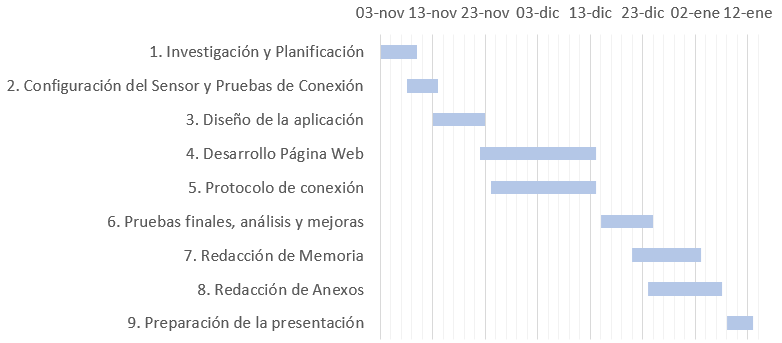
\includegraphics[width=1\textwidth]{img/A2_PlanTemporal/Gantt_Inicial.png}
    \caption{Diagrama de Gantt inicial}
    \label{fig:gantt1}
\end{figure}

\begin{figure}[h]
    \centering
    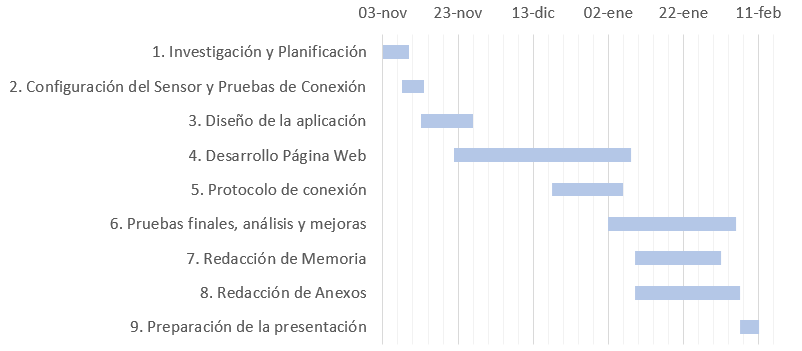
\includegraphics[width=1\textwidth]{img/A2_PlanTemporal/Gantt_Final.png}
    \caption{Diagrama de Gantt final}
    \label{fig:gantt2}
\end{figure}


\section{Planificación económica}
En una planificación económica realista hay que considerar todos los costes de realización del proyecto. Esto incluye desde la valoración económica de herramientas de desarrollo software hasta la de materiales, equipos y sueldos del personal necesario.
Además de los costos, también se debe tener en cuenta la rentabilidad a través de diversas opciones de explotación.

En este apartado se presenta la planificación económica del proyecto realizado. Se incluye el desarrollo software de la página web y el montaje hardware de un prototipo anterior sobre el que se han realizado modificaciones.

\subsection{Coste de personal}
Ha habido únicamente una persona involucrada en el proyecto, desde el desarrollo hasta el diseño, que para el cálculo de los costos de contratación será considerada Ingeniero de la Salud sin experiencia. 
En España, un Ingeniero Biomédico recién egresado o con menos de 3 años de experiencia, que es la situación que más se ajusta a este caso, puede aspirar a un salario medio bruto de 29.020 €/año \cite{jobtedIngenieroBiomedico}. Teniendo en cuenta que el contrato necesario para la realización de esté proyecto debe ser de 2 meses de duración a jornada completa, el costo del empleado será de 4.836,66 €, cantidad a la que habrá que añadirle el pago de la Seguridad Social que corre a cargo de la empresa. La cantidad de dinero a pagar según el Régimen General de la Seguridad Social \cite{SeguridaSocial:online} se puede calcular a través de unos porcentajes a aplicar sobre el salario bruto como se muestra en la Tabla \ref{tab: costesEmpleado}.

\begin{table}[]
    \centering
    \begin{tabular}{lll}
        \hline
        \rowcolor[HTML]{FFFFFF} 
        \textbf{Sueldo bruto (€/mes)} & 2.418,33 \\ \hline
        \rowcolor[HTML]{EFEFEF} 
        \multicolumn{2}{|c|}{\textbf{Costes del Régimen General de la Seguridad Social}} \\ \hline
        \rowcolor[HTML]{FFFFFF} 
        Contingencias Comunes (23,60\%) & 570,72 \\ \hline
        \rowcolor[HTML]{EFEFEF} 
        Contrato duración determinada Tiempo Completo (6,7\%) & 162,02 \\ \hline
        \rowcolor[HTML]{FFFFFF} 
        FOGASA (0,2\%) & 4,83 \\ \hline
        \rowcolor[HTML]{EFEFEF} 
        Formación Profesional (0,6\%) & 14,51 \\ \hline
        \rowcolor[HTML]{FFFFFF} 
        \textbf{Costo total - 1 mes} & \textbf{3.170,41} \\ \hline
        \rowcolor[HTML]{C0C0C0} 
        \textbf{Costo total - 2 meses} & \textbf{6.340,82 €} \\ \hline
    \end{tabular}
    \caption{Desglose de costes de contratación}
    \label{tab: costesEmpleado}
\end{table}

\subsection{Costes de software}
Todas las herramientas software empleadas compartían la característica de ser de código abierto y gratuitas. Visual Studio Code, XAMPP, Node.js y Arduino IDE han sido algunas de las utilizadas.

\subsection{Amortización de los equipos}
El único equipo indispensable para el desarrollo del proyecto ha sido un portátil de la marca HP (modelo HP Pavillion Laptop 15-cs2xxx), cuyo precio de compra fue de 849,45€ y al que se le estima una vida útil de 6 años. La amortización \footnote{Amortización es la pérdida de valor de un bien o activo a lo largo del tiempo.} del portatil durante los dos meses y medio que duró el trabajo puede calcularse aplicando la fórmula de la Figura \ref{fig:amortizacion-portatil} , obteniendo como resultado 29,49 € \cite{Amortizacion:online}.

\begin{figure}[h]
    \centering
    \[
    \text{Amortización del Periodo} = \frac{\text{Precio de Compra}}{\text{Vida Útil en Años}} \times \frac{\text{Meses de Uso}}{12}
    \]
    \caption{Fórmula para el Cálculo de la Amortización durante un Periodo Determinado}
    \label{fig:amortizacion-portatil}
\end{figure}

\subsection{Costes de hardware}
Se va a estimar el precio del prototipo empleado para la realización de pruebas a lo largo del proyecto. En este caso el cálculo de costos se ha limitado al único dispositivo que todavía requiere mejoras pero, si se obtuviera un producto final susceptible de lanzamiento al mercado, además del cálculo del coste por unidad habría que realizar una estimación de la cantidad necesaria de cada material para la producción del número de dispositivos que se pretenda distribuir.\\
Tras la búsqueda y comparación de precios para los componentes necesarios en las tiendas online de Amazon, turiBOT y AliExpress, se concluye que AliExpress ofrece los mejores precios. Sin embargo, debido a los problemas reportados con su distribuidora en España, se ha descartado esta opción. Los precios de Amazon \cite{Amazones75:online} y turiBOT \cite{turi:online} son bastante similares, por lo que se ha optado por elaborar el presupuesto considerando a ambas empresas. Los resultados se pueden visualizar en la Tabla \ref{tab:costesComponentes}.

\begin{table}[]
    \centering
    \begin{tabular}{ll}
        \hline
        \rowcolor[HTML]{FFFFFF} 
        \textbf{Componente} & \textbf{Coste (€)} \\ \hline
        \rowcolor[HTML]{EFEFEF} 
        Microprocesador Arduino UNO R3 & 24,68 \\ \hline
        \rowcolor[HTML]{FFFFFF} 
        Cables & 1,57 \\ \hline
        \rowcolor[HTML]{EFEFEF} 
        Acelerómetro + Giroscopio MPU-6050 & 3,92 \\ \hline
        \rowcolor[HTML]{FFFFFF} 
        Módulo bluetooth HC-05 & 10,00 \\ \hline
        \rowcolor[HTML]{EFEFEF} 
        Display LCD 16x2 & 7,5 \\ \hline
        \rowcolor[HTML]{FFFFFF} 
        Módulo I2C & 2,66 \\ \hline
        \rowcolor[HTML]{EFEFEF} 
        2 pulsadores & 0,50 \\ \hline
        \rowcolor[HTML]{FFFFFF} 
        2 resistencias & 0,50 \\ \hline
        \rowcolor[HTML]{EFEFEF} 
        Caja para prototipos & 7,00 \\ \hline
        \rowcolor[HTML]{FFFFFF} 
        Batería recargable 9V & 10,00 \\ \hline
        \rowcolor[HTML]{EFEFEF} 
        Conector para batería & 0,35 \\ \hline
        \rowcolor[HTML]{FFFFFF} 
        Cable multihilo flexible & 11,99 \\ \hline
        \rowcolor[HTML]{EFEFEF} 
        Interruptor & 1,19 \\ \hline
        \rowcolor[HTML]{FFFFFF} 
        Proto shield Arduino & 3,19 \\ \hline
        \rowcolor[HTML]{EFEFEF} 
        Conector 5 pines macho-hembra & 6,99 \\ \hline
        \rowcolor[HTML]{C0C0C0} 
        \textbf{Coste Total} & \textbf{92,04 €} \\ \hline
    \end{tabular}
    \caption{Desglose de costes de los componentes}
    \label{tab:costesComponentes}
\end{table}


\section{Viabilidad legal}
En el desarrollo de este proyecto tecnológico, es crucial considerar su viabilidad legal para garantizar no solo la protección del proceso y del producto intelectual, sino también el cumplimiento de las regulaciones vigentes.

\subsection{Leyes y normativas}
 La normativa de interés en el desarrollo de un proyecto como el que se presenta, debe abarcar aspectos como la comercialización y derechos de los usuarios. Su cumplimiento va asegurar la calidad y seguridad del producto y su desarrollo, fortaleciendo la confianza de todas las partes involucradas.
Considerando el marco legislativo europeo y español, se procede a describir los principales decretos y leyes que afectan al proyecto.

\subsubsection{Protección de datos personales y respeto de la privacidad}
Los datos personales deben ser protegidos debido a su valor e importancia, respetando siempre el derecho de las personas a la transparencia en el tratamiento de sus datos. En este caso se trabaja con datos que podrían ser considerados sanitarios, lo que les confiere un caracter más sensible. Aunque hasta el momento no se han empleado datos reales de pacientes ni realizado evaluaciones sobre su evolución, en el futuro las siguienes leyes marcarán cómo se debe realizar dicho tratamiento.

\begin{itemize}
    \item Reglamento (UE) 2016/679 (Reglamento general de protección de datos, RGPD), aprobado por el Parlamento y Consejo Europeo, establece el marco legal para el desarrollo del tratamiento y la libre circulación de los datos de personas físicas, a las que reserva el derecho de acceso, rectificación y eliminación de sus datos \cite{BOE_RGPD:online}.
    \item Ley Orgánica 3/2018 de Proteccióon de Datos Personales y garantía de los derechos digitales (LOPDGDD). Esta ley complementa el RGPD en España estableciendo y regulando aspectos que este último no llegaba a concretar, ya que delegaba la oportunidad de hacerlo a cada Estado miembro, como es el caso de los datos en el ámbito digital\cite{BOE_LOPDGDD:online} \cite{BOE_RGPD:online}.
    \item La Ley 41/2002 básica reguladora de la autonomía del paciene y de derechos y obligaciones en materia de información y documentación clínica \cite{BOE_41/2002:online}, defiende los derechos básicos de los pacientes, entre los que se encuentra la confidencialidad.
\end{itemize}

\subsubsection{Comercialización de dispositivos médicos}
La alta sensibilidad del ámbito sanitario se tiene en cuenta a través de esta normativa que garantiza la seguridad, eficacia y calidad de los productos destinados a emplearse en este campo.
\begin{itemize}
    \item El Reglamento (UE) 2017/745 sobre los productos sanitarios \cite{BOE_2017/745:online} especifica toda una serie de factores a tener en cuenta para la garantizar la seguridad de los dispositivos y permite que sean los Estados miembro quienes decidan qué es considerado producto sanitario. Añade que los programas informáticos serán considerados productos sanitarios según la función a la que estén destinados. En el caso de la web que se desarrolla en este proyecto, que todavía está en una etapa muy temprana, el enfoque que se le ha dado para que esté destinada al seguimiento y adaptación del tratamiento, la convertiría en un producto sanitario.
    \item El marcado CE (Conformidad Europea) que indica que el producto cumple con todos los requirimientos, permite que los productos sanitarios disfruten de la libre circulación dentro de la Unión como se describe en el Reglamento 2017/745 \cite{BOE_2017/745:online}, donde también se describe cómo debe realizarse y en qué casos.
    \item Real Decreto 192/2023 por el que se regulan los productos sanitarios \cite{BOE_192/2023:online}. Hace responsable a la Agencia Española de Medicamentos y Productos Sanitarios de decir sobre la clasificación de cada producto y de proporcionar o retirar las licencias pertinentes.
\end{itemize}

\subsubsection{Derechos de autor y propiedad intelectual}
Tanto en España como en la Unión Europea existe un conjunto de leyes y regulaciones relacionadas con los derechos de autor y propiedad intelectual aplicables a la protección de software.
\begin{itemize}
    \item Directiva (UE) 2009/24/CE sobre la protección jurídica de programas de ordenador \cite{BOE_2009/24/CE:online}. Establece que los programas de ordenador de cualquier tipo, incluso los incorporados en el hardware (como el que en este proyecto se carga en el microprocesador Arduino), están protegidos por los derechos de autor. Además, describe los criterios para determinar si se trata de una obra original entre otros aspectos relevantes.
    \item Real Decreto Legislativo 1/1996 por el que se aprueba el texto refundido de la Ley de Propiedad Intelectual \cite{BOE_1/1996:online}. En el, se definen las bases de la propiedad intelectual y se describen las características y condiciones de los derechos de autor.
\end{itemize}

\subsection{Licencias de software}
Las licencias de software son una especie de contrato entre el propietario y el usuario interesado, en el que se establecen los términos, cláusulas y responsabilidades que se deben cumplir para respetar los derechos de ambas partes \cite{TiposdelLicencias:online}.

\subsubsection{Licencias de softwares empleados en este proyecto}
Se ha hecho uso de una amplia gama de herramientas, todas ellas protegidas con algún tipo de licencia que habría que tener en cuenta a la hora de la distribución de nuestro proyecto. En la tabla \ref{tab:licencias} se muestran, agrupadas en categorías, todas las herramientas software junto a sus respectivas licencias.

\begin{table}[]
    \begin{tabular}{|c|l|l|}
    \hline
    \rowcolor[HTML]{FFFFFF} 
    \multicolumn{1}{|l|}{\cellcolor[HTML]{FFFFFF}\textbf{Categoría}} & \textbf{Herramienta} & \textbf{Tipo de Licencia} \\ \hline 
    \rowcolor[HTML]{EFEFEF} 
    \cellcolor[HTML]{EFEFEF}   & Arduino IDE & GLP/LGPL  \\ \cline{2-3}
    \rowcolor[HTML]{EFEFEF} 
    \multirow{-2}{*}{\cellcolor[HTML]{EFEFEF}\begin{tabular}[c]{@{}c@{}}IDEs\end{tabular}} & Visual Studio Code   & MIT License\\ \hline
    \rowcolor[HTML]{FFFFFF} 
    \begin{tabular}[c]{@{}c@{}}Gestión Bases\\ de Datos\end{tabular}  & MySQL, XAMPP & GPL \\ \hline
    \rowcolor[HTML]{EFEFEF} 
    \cellcolor[HTML]{EFEFEF}    & I2Cdev, MPU6050  & MIT License  \\ \cline{2-3} 
    \rowcolor[HTML]{EFEFEF} 
    \cellcolor[HTML]{EFEFEF}    & Wire, SoftwareSerial & LGPL/GPL \\ \cline{2-3}
    \rowcolor[HTML]{EFEFEF}
    \multirow{-3}{*}{\cellcolor[HTML]{EFEFEF} Librerías Arduino} & LiquidCrystal\_I2C & Libre  \\ \hline
    \rowcolor[HTML]{FFFFFF} 
    \cellcolor[HTML]{FFFFFF} & PySerial & BSD License \\ \cline{2-3} 
    \rowcolor[HTML]{FFFFFF} 
    \multirow{-3}{*}{\cellcolor[HTML]{FFFFFF}Paquetes Python} & Requests & Apache License 2.0 \\ \hline
    \rowcolor[HTML]{EFEFEF} 
    Paquetes Node.js & \begin{tabular}[c]{@{}l@{}}Express, MySQL,\\ Body-Parser, CORS\end{tabular} & MIT License               \\ \hline
    \rowcolor[HTML]{FFFFFF} 
    \cellcolor[HTML]{FFFFFF}  & Draw.io & Apache License 2.0 \\ \cline{2-3} 
    \rowcolor[HTML]{FFFFFF} 
    \multirow{-2}{*}{\cellcolor[HTML]{FFFFFF}Diseño} & Balsamiq Wireframes & Licencia Propietario \\ \hline
    \end{tabular}
    \caption{Herramientas empleadas y sus licencias}
    \label{tab:licencias}
\end{table}

\subsubsection{Licencia de este proyecto}
Para este proyecto se ha seleccionado la Licencia Apache 2.0. Esta licencia de software libre y código abierto, que destaca por las escasas restricciones, no proporciona ningún tipo de garantía ni establece restricciones de uso \cite{ApacheLi71:online}. No obstante, su cumplimiento de los requisitos mínimos y que no supone ningún coste adicional, han sido razones suficientes para su selección.
